% !TEX TS-program = pdflatex
\documentclass[11pt]{article}

% -------------------- Packages --------------------
\usepackage[a4paper,margin=1in]{geometry}
\usepackage{amsmath,amssymb}
\usepackage[T1]{fontenc}
\usepackage{lmodern}
\usepackage{xcolor}
\usepackage{tcolorbox}
\tcbuselibrary{skins,breakable}
\usepackage{enumitem}
\usepackage{hyperref}
\usepackage{tikz}
\usetikzlibrary{arrows.meta,positioning,calc}

\pagestyle{empty}

% -------------------- Dark Theme Colors --------------------
\definecolor{bg}{HTML}{000000}
\definecolor{pairbg}{HTML}{121212}
\definecolor{solbg}{HTML}{0A0A0A}
\definecolor{border}{HTML}{2A2A2A}
\definecolor{text}{HTML}{FFFFFF}
\definecolor{muted}{HTML}{C9CDD3}
\definecolor{gold}{HTML}{FFD700}
\definecolor{green}{HTML}{4ADE80}
\definecolor{cyan}{HTML}{38BDF8}

\pagecolor{bg}
\color{text}

\hypersetup{
  colorlinks=true,
  linkcolor=cyan,
  urlcolor=cyan
}

\setlength{\parindent}{0pt}
\setlength{\parskip}{10pt}

\setlist[itemize]{left=1.4em,itemsep=6pt,topsep=6pt}
\setlist[enumerate]{left=1.6em,itemsep=4pt,topsep=4pt}

% -------------------- tcolorbox Base --------------------
\tcbset{
  enhanced,
  breakable,
  arc=12pt,
  boxrule=0.8pt,
  left=16pt,right=16pt,top=12pt,bottom=12pt,
  % prevents right-side overflow for long text lines
  before upper=\sloppy\setlength{\emergencystretch}{2em}
}

\newtcolorbox{QAPair}[1]{%
  colback=pairbg,
  colbacklower=solbg,
  colframe=border,
  coltext=text,
  title=\textcolor{gold}{\bfseries #1},
  fonttitle=\bfseries,
  coltitle=text,
  segmentation style={draw=border, dashed, line width=0.6pt},
}

\newtcolorbox{QuickBox}{%
  colback=pairbg,
  colframe=cyan,
  coltext=text,
  fontupper=\color{text},
  borderline north={4pt}{0pt}{cyan},
  arc=14pt,
  boxrule=0.8pt
}

% Helper for step headings
\newcommand{\Step}[1]{\textcolor{muted}{\textbf{Step #1:}}}

% Small helper text
\newcommand{\Note}[1]{\textcolor{muted}{#1}}

% -------- Step + multi-line equations helper (READABLE) -----
% Usage:
% \StepEq{1}{
%   f(1) &= 0\\
%   \Rightarrow\ t-a &= 0
% }
\newcommand{\StepEq}[2]{%
  \Step{#1}\par
  \vspace{-6pt}
  \begin{align*}
    #2
  \end{align*}
  \vspace{-10pt}
}

% -------------------- TikZ Styles --------------------
\tikzset{
  setoval/.style={draw=muted, line width=0.9pt},
  elem/.style={text=text, font=\small},
  setname/.style={text=text, font=\bfseries\small},
  maplabel/.style={text=muted, font=\small\itshape},
  maparr/.style={-{Latex[length=3mm]}, draw=cyan, line width=1.1pt}
}

% ============================================================
\begin{document}

\begin{center}
{\LARGE\bfseries \textcolor{gold}{Exercise 6.1 --- Solutions}}\\[-2pt]
\end{center}

\begin{QuickBox}
{\color{cyan}\bfseries Quick notes (functions)}\par\medskip
\begin{itemize}
\item A relation $R\subseteq A\times B$ is a \textbf{function} $A\to B$ iff \textbf{every} $a\in A$ appears \textbf{exactly once} as a first component $(a,b)$.
\item \textbf{One-one (injective):} different inputs give different outputs.
\item \textbf{Onto (surjective):} every element of codomain has at least one preimage.
\item \textbf{Many-one:} two (or more) different inputs map to the same output.
\item \textbf{Bijective:} both one-one and onto.
\end{itemize}
\end{QuickBox}

% ============================================================
% Q1
\begin{QAPair}{Question 1}
\textcolor{gold}{\bfseries Question:}
If $A=\{2,4,6,8\}$ and $B=\{1,3,5\}$, which of the following relations are functions from $A$ to $B$?
\[
\begin{aligned}
\text{(i)}\; R_1&=\{(2,3),(6,5),(8,3),(4,1)\},\\
\text{(ii)}\; R_2&=\{(2,3),(6,1),(8,3),(6,5)\},\\
\text{(iii)}\; R_3&=\{(2,3),(6,5),(8,3)\},\\
\text{(iv)}\; R_4&=\{(2,3),(6,3),(8,3),(4,1)\}.
\end{aligned}
\]
\tcblower
\textcolor{green}{\bfseries Answer:}\par
\Note{A relation is a function $A\to B$ iff each of $2,4,6,8$ appears \textbf{exactly once} as a first component.}\par\medskip

\Step{1} $R_1$: $2,4,6,8$ each appear once $\Rightarrow$ $R_1$ is a function.\par
\Step{2} $R_2$: $6$ appears twice: $(6,1)$ and $(6,5)$ $\Rightarrow$ not a function.\par
\Step{3} $R_3$: $4$ does not appear at all $\Rightarrow$ not a function from $A$ to $B$.\par
\Step{4} $R_4$: $2,4,6,8$ each appear once $\Rightarrow$ $R_4$ is a function.\par

\[
\boxed{\;R_1 \text{ and } R_4 \text{ are functions from }A\text{ to }B.\;}
\]
\end{QAPair}

% ============================================================
% Q2
\begin{QAPair}{Question 2}
\textcolor{gold}{\bfseries Question:} Identify the functions from the following diagrams. Also write their type.
\tcblower
\textcolor{green}{\bfseries Answer:}

\textcolor{gold}{\bfseries (i)} \quad From the diagram we read
\[
f:\{2,3,5\}\to\{1,3,5\},\qquad f(2)=3,\; f(3)=5,\; f(5)=1.
\]

\begin{center}
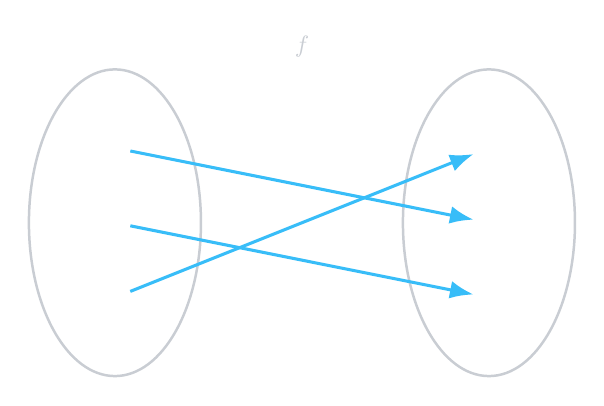
\begin{tikzpicture}[font=\small, scale=0.95, transform shape]
  % Ovals (taller + label inside)
  \draw[setoval] (0,-1.6) ellipse (1.15 and 2.05);
  \draw[setoval] (5,-1.6) ellipse (1.15 and 2.05);

  \node[setname] at (0,0.05) {A};
  \node[setname] at (5,0.05) {B};

  \node[elem] (a2) at (0,-0.6) {$2$};
  \node[elem] (a3) at (0,-1.6) {$3$};
  \node[elem] (a5) at (0,-2.6) {$5$};

  \node[elem] (b1) at (5,-0.6) {$1$};
  \node[elem] (b3) at (5,-1.6) {$3$};
  \node[elem] (b5) at (5,-2.6) {$5$};

  \draw[maparr] (a2) -- (b3);
  \draw[maparr] (a3) -- (b5);
  \draw[maparr] (a5) -- (b1);

  \node[maplabel] at (2.5,0.75) {$f$};
\end{tikzpicture}
\end{center}

\Step{1} Each input has exactly one output, so it \emph{is} a function.\par
\Step{2} All outputs $\{1,3,5\}$ are hit and outputs are distinct $\Rightarrow$
$\boxed{\text{bijective (one-one and onto)}}$.\par

\vspace{6pt}
\textcolor{gold}{\bfseries (ii)} \quad In the diagram, $4\in P$ has \textbf{no arrow} (no image), so it is \textbf{not} a function.

\begin{center}
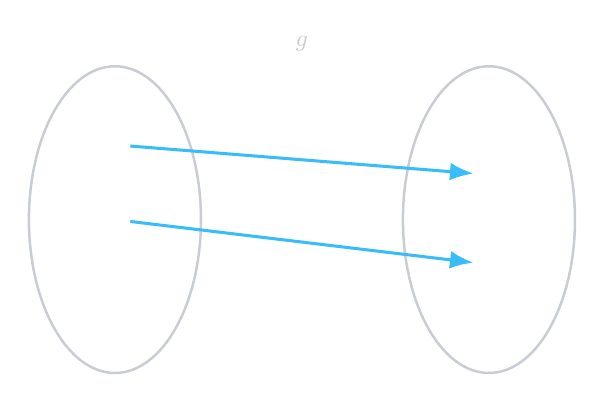
\begin{tikzpicture}[font=\small, scale=0.95, transform shape]
  \draw[setoval] (0,-1.6) ellipse (1.15 and 2.05);
  \draw[setoval] (5,-1.6) ellipse (1.15 and 2.05);

  \node[setname] at (0,0.05) {P};
  \node[setname] at (5,0.05) {Q};

  \node[elem] (p0) at (0,-0.6) {$0$};
  \node[elem] (p2) at (0,-1.6) {$2$};
  \node[elem] (p4) at (0,-2.6) {$4$};

  \node[elem] (q5) at (5,-1.0) {$5$};
  \node[elem] (q7) at (5,-2.2) {$7$};

  \draw[maparr] (p0) -- (q5);
  \draw[maparr] (p2) -- (q7);

  \node[maplabel] at (2.5,0.75) {$g$};
\end{tikzpicture}
\end{center}

\[
\boxed{\text{(ii) is not a function (an element of the domain has no image).}}
\]

\vspace{6pt}
\textcolor{gold}{\bfseries (iii)} \quad From the diagram we read
\[
h:\{0,2,4\}\to\{a,b,c\},\qquad h(0)=b,\; h(2)=c,\; h(4)=c.
\]

\begin{center}
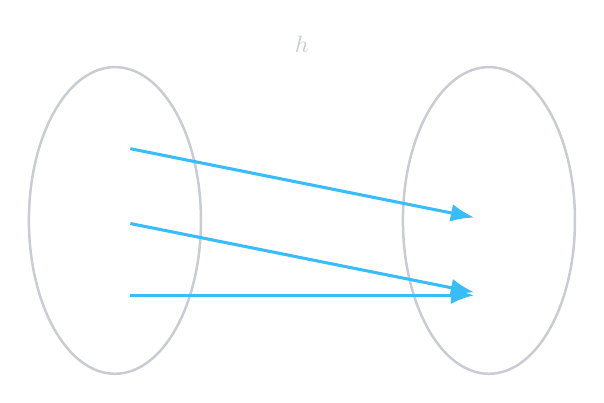
\begin{tikzpicture}[font=\small, scale=0.95, transform shape]
  \draw[setoval] (0,-1.6) ellipse (1.15 and 2.05);
  \draw[setoval] (5,-1.6) ellipse (1.15 and 2.05);

  \node[setname] at (0,0.05) {X};
  \node[setname] at (5,0.05) {Y};

  \node[elem] (x0) at (0,-0.6) {$0$};
  \node[elem] (x2) at (0,-1.6) {$2$};
  \node[elem] (x4) at (0,-2.6) {$4$};

  \node[elem] (ya) at (5,-0.6) {$a$};
  \node[elem] (yb) at (5,-1.6) {$b$};
  \node[elem] (yc) at (5,-2.6) {$c$};

  \draw[maparr] (x0) -- (yb);
  \draw[maparr] (x2) -- (yc);
  \draw[maparr] (x4) -- (yc);

  \node[maplabel] at (2.5,0.75) {$h$};
\end{tikzpicture}
\end{center}

\Step{1} Each input has exactly one output, so it \emph{is} a function.\par
\Step{2} $2$ and $4$ both map to $c$ $\Rightarrow$ $\boxed{\text{many-one}}$.\;
Also $a$ is not hit $\Rightarrow$ $\boxed{\text{into (not onto)}}$.\par
\end{QAPair}

% ============================================================
% Q3
\begin{QAPair}{Question 3}
\textcolor{gold}{\bfseries Question:}
If $f(x)=x^2-\dfrac12 x+3$, evaluate: (i) $f(2)$ (ii) $f(-1)$ (iii) $f\!\left(\dfrac23\right)$ (iv) $f(t+1)$.
\tcblower
\textcolor{green}{\bfseries Answer:}

\textcolor{gold}{\bfseries (i) $f(2)$}\par
\StepEq{1}{
f(2) &= 2^2-\frac12(2)+3\\
     &= 4-1+3\\
     &= 6
}
\[
\boxed{f(2)=6}
\]

\textcolor{gold}{\bfseries (ii) $f(-1)$}\par
\StepEq{1}{
f(-1) &= (-1)^2-\frac12(-1)+3\\
      &= 1+\frac12+3\\
      &= \frac{9}{2}
}
\[
\boxed{f(-1)=\frac{9}{2}}
\]

\textcolor{gold}{\bfseries (iii) $f\!\left(\dfrac23\right)$}\par
\StepEq{1}{
f\!\left(\frac23\right) &= \left(\frac23\right)^2-\frac12\left(\frac23\right)+3\\
&= \frac{4}{9}-\frac{1}{3}+3\\
&= \frac{4}{9}-\frac{3}{9}+3\\
&= \frac{1}{9}+3\\
&= \frac{28}{9}
}
\[
\boxed{f\!\left(\frac23\right)=\frac{28}{9}}
\]

\textcolor{gold}{\bfseries (iv) $f(t+1)$}\par
\StepEq{1}{
f(t+1) &= (t+1)^2-\frac12(t+1)+3\\
&= t^2+2t+1-\frac{t}{2}-\frac12+3\\
&= t^2+\frac{3}{2}t+\frac{7}{2}
}
\[
\boxed{f(t+1)=t^2+\frac{3}{2}t+\frac{7}{2}}
\]
\end{QAPair}

% ============================================================
% Q4
\begin{QAPair}{Question 4}
\textcolor{gold}{\bfseries Question:}
If $X=$ set of prime factors of $6$ and $Y=$ set of first three non-negative integers, check whether the function
$f:X\to Y=\{(x,y)\mid x-y=1\}$ is injective or bijective.
\tcblower
\textcolor{green}{\bfseries Answer:}\par

\StepEq{1}{
X &= \{2,3\},\qquad Y=\{0,1,2\}
}
\StepEq{2}{
x-y &= 1 \Rightarrow y=x-1
}
\StepEq{3}{
f(2) &= 1,\quad f(3)=2 \Rightarrow \text{Range}(f)=\{1,2\}
}

\Step{4} Injective: $2\neq 3 \Rightarrow f(2)\neq f(3)$ $\Rightarrow$ $\boxed{\text{injective}}$.\par
\Step{5} Not onto: $0\in Y$ is not in the range $\Rightarrow$ $\boxed{\text{not bijective}}$.\par

\[
\boxed{\text{The function is injective but not bijective.}}
\]
\end{QAPair}

% ============================================================
% Q5
\begin{QAPair}{Question 5}
\textcolor{gold}{\bfseries Question:}
A function is defined by $f(x)=t-ax$. Find $a$ and $t$ if $0$ and $2$ are the images of $1$ and $-1$ respectively.
\tcblower
\textcolor{green}{\bfseries Answer:}\par

\StepEq{1}{
f(1) &= 0\\
\Rightarrow\ t-a(1) &= 0\\
\Rightarrow\ t-a &= 0\\
\Rightarrow\ t &= a
}

\StepEq{2}{
f(-1) &= 2\\
\Rightarrow\ t-a(-1) &= 2\\
\Rightarrow\ t+a &= 2
}

\StepEq{3}{
\text{Substitute } t=a:\quad a+a &= 2\\
2a &= 2\\
a &= 1
}

\StepEq{4}{
t &= a = 1
}

\[
\boxed{a=1,\;\; t=1.}
\]
\end{QAPair}

% ============================================================
% Q6
\begin{QAPair}{Question 6}
\textcolor{gold}{\bfseries Question:}
A function is defined by $f(x)=mx+c$. Is $f$ bijective? Justify your answer.
\tcblower
\textcolor{green}{\bfseries Answer:}\par
\Note{(Standard case: domain $\mathbb{R}$ and codomain $\mathbb{R}$.)}\par\medskip

\Step{1} If $m\neq 0$, then $f(x)=mx+c$ is strictly monotone, so it is \textbf{one-one} (injective).\par

\Step{2} If $m\neq 0$, then for any $y\in\mathbb{R}$ choose
\[
x=\frac{y-c}{m}.
\]
Then $f(x)=y$, so $f$ is \textbf{onto} (surjective).\par

\Step{3} Therefore,
\[
\boxed{\text{$f$ is bijective iff } m\neq 0.}
\]

\Step{4} If $m=0$, then $f(x)=c$ is a constant function, so it is \textbf{not one-one} and \textbf{not onto}
(unless the codomain is exactly $\{c\}$).\par
\end{QAPair}

\end{document}
